\section{Results}
\label{sec:results}

We organize our results around three experiments: representational decay
curves (\secref{sec:decay_curves}), the comparison between autoregressive and
teacher-forced conditions (\secref{sec:ar_vs_tf}), and ablation studies
(\secref{sec:ablations}).

\subsection{Experiment 1: Representational Decay Is Instantaneous}
\label{sec:decay_curves}

\Figref{fig:decay} shows the cosine similarity delta ($\Delta$cos) between
steered and unsteered hidden states at the injection layer across token
positions. During steering (positions $-3$ to $-1$), the delta is stable at
approximately $+0.019$ for the truthful direction, confirming that the steering
vector produces a consistent representational shift. At position~0---the first
token generated without the steering vector---the delta drops to ${\sim}0.000$
and remains there for all subsequent tokens.

\begin{figure}[t]
    \centering
    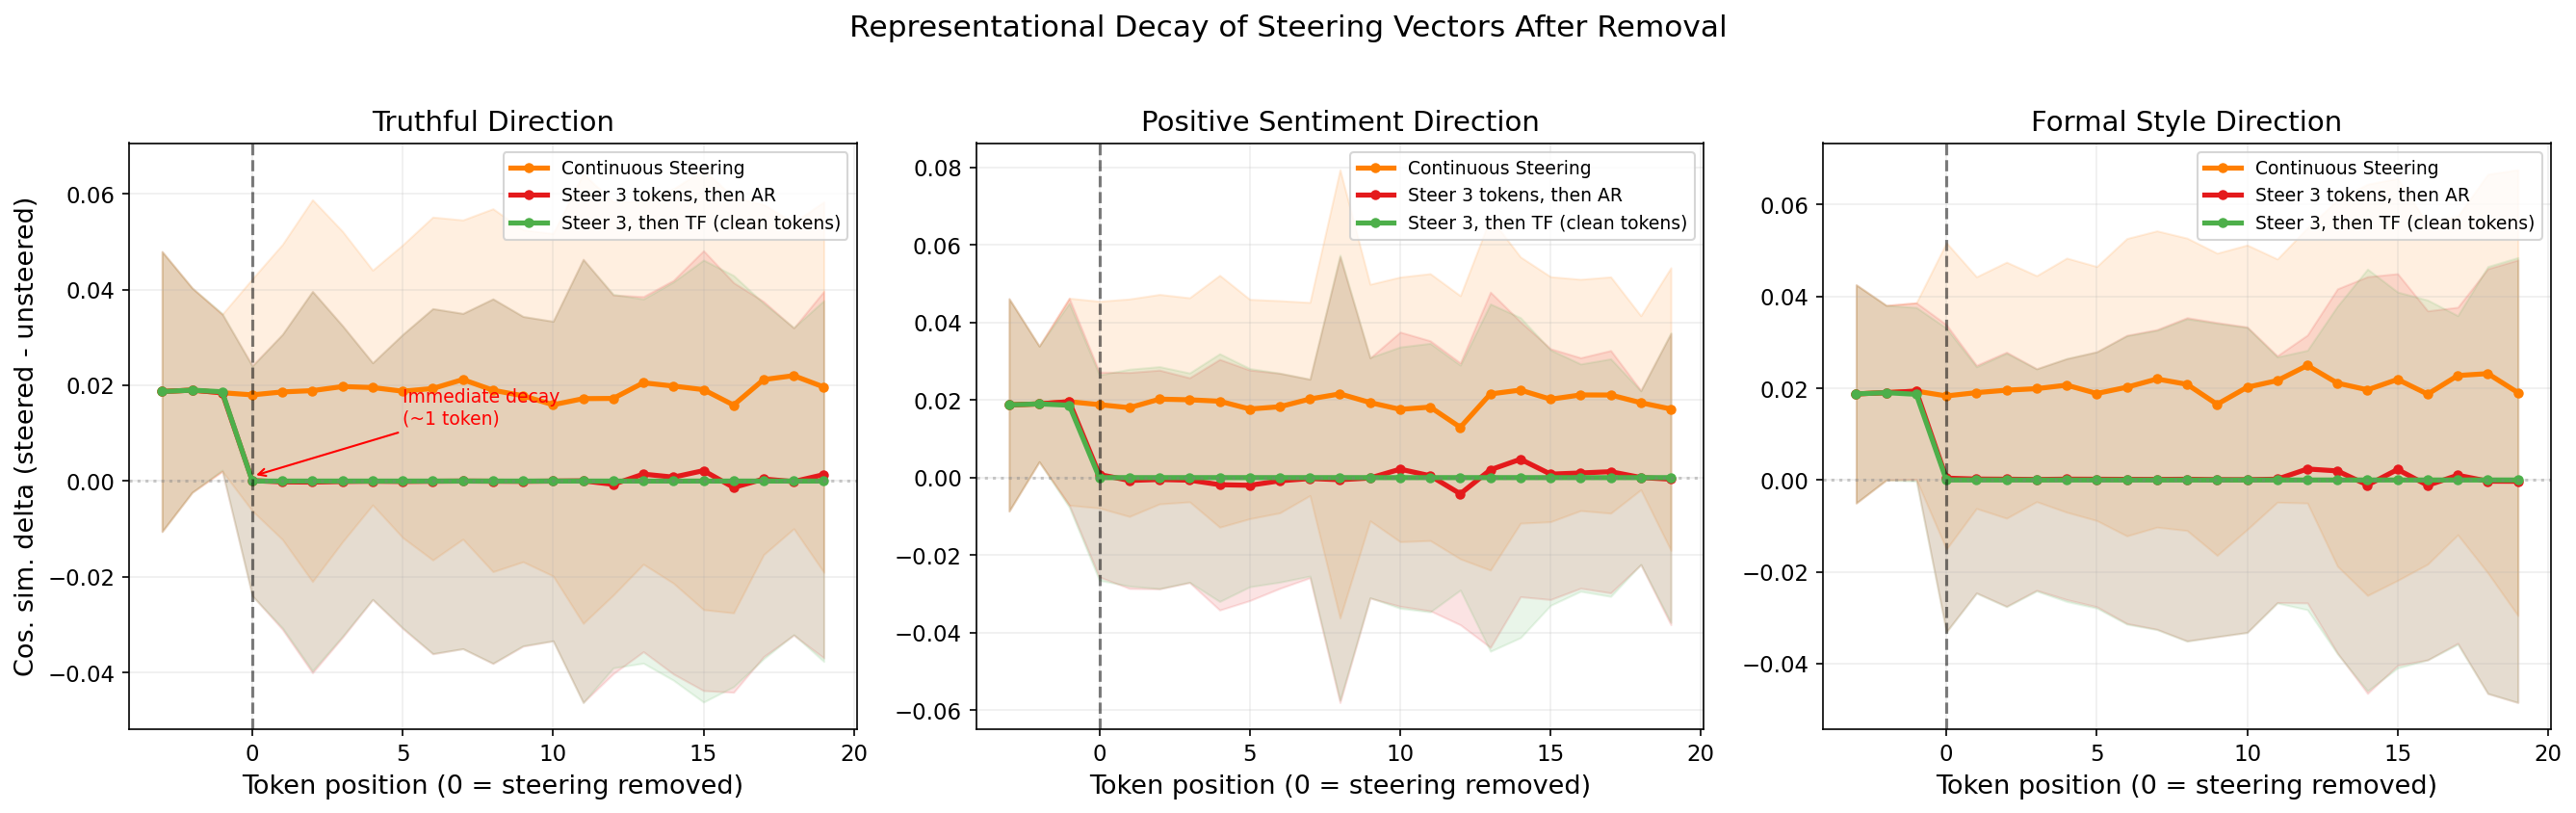
\includegraphics[width=0.95\linewidth]{figures/key_finding_representational_decay.png}
    \caption{Cosine similarity delta ($\Delta$cos) between steered and unsteered
    hidden states at the injection layer (layer~24) across token positions.
    Steering is applied at positions $-3$ to $-1$ (shaded region) and removed
    at position~0. The delta drops from ${\sim}0.019$ to ${\sim}0.000$ within a
    single generation step, indicating instantaneous representational decay.
    Results are averaged over 20 prompts with the truthful steering direction.}
    \label{fig:decay}
\end{figure}

\Tabref{tab:decay_values} presents the raw delta values for the truthful
direction across representative token positions. The continuous steering
condition maintains a stable delta of ${\sim}0.018$ throughout, while the
\AR condition shows a delta indistinguishable from zero at every post-removal
position. The \TFclean condition, which feeds unsteered tokens after the
steering period, shows the same instantaneous reversion.

\begin{table}[t]
    \centering
    \caption{Cosine similarity delta ($\Delta$cos) at the injection layer for
    the truthful steering direction. Steering is applied at positions $-3$ to
    $-1$ and removed at position~0. Values are averaged over 20 prompts.
    The \AR and \TFclean conditions revert to
    zero within a single step.}
    \label{tab:decay_values}
    \begin{tabular}{@{}lrrr@{}}
        \toprule
        Position & Continuous & \AR & \TFclean \\
        \midrule
        $-3$ (steered) & $+0.0187$ & $+0.0187$ & $+0.0187$ \\
        $-2$ (steered) & $+0.0190$ & $+0.0190$ & $+0.0190$ \\
        $-1$ (steered) & $+0.0184$ & $+0.0184$ & $+0.0184$ \\
        \midrule
        $\phantom{-}0$ (first unsteered) & $+0.0181$ & $\mathbf{+0.0001}$ & $\mathbf{+0.0000}$ \\
        $\phantom{-}1$ & $+0.0186$ & $\mathbf{-0.0002}$ & $\mathbf{+0.0000}$ \\
        $\phantom{-}5$ & $+0.0188$ & $\mathbf{-0.0001}$ & $\mathbf{-0.0001}$ \\
        $10$ & $+0.0160$ & $\mathbf{+0.0000}$ & $\mathbf{-0.0001}$ \\
        $19$ & $+0.0197$ & $\mathbf{+0.0013}$ & $\mathbf{-0.0001}$ \\
        \bottomrule
    \end{tabular}
\end{table}

This pattern is consistent across all three behavioral dimensions. The positive
sentiment and formal style directions show the same instantaneous decay, with
deltas dropping from comparable magnitudes to values indistinguishable from zero
at position~0.

\subsection{Experiment 2: Autoregressive vs.\ Teacher-Forced}
\label{sec:ar_vs_tf}

\para{Are hidden states different when we replay steered tokens without the
vector?} No. \Tabref{tab:ar_vs_tf} compares the \AR and \TF conditions across
both representational (cosine similarity delta) and behavioral (KL divergence)
metrics. The two conditions produce \emph{exactly identical} hidden states and
output distributions, with Cohen's $d = 0.000$ for all metrics. This means
that teacher-forcing the same steered tokens---without the steering
vector---produces the same internal representations as autoregressive generation.
The model retains no hidden state memory of the steering intervention.

\begin{table}[t]
    \centering
    \caption{Comparison of \AR, \TF, and \TFclean conditions. \AR and \TF
    produce identical hidden states (Cohen's $d = 0.000$). \TFclean shows
    complete reversion to the unsteered baseline. KL divergence from unsteered
    is averaged over post-removal positions. $p$-values from paired $t$-tests.}
    \label{tab:ar_vs_tf}
    \begin{tabular}{@{}llrr@{}}
        \toprule
        Comparison & Metric & $p$-value & Cohen's $d$ \\
        \midrule
        \AR vs.\ \TF & $\Delta$cos & --- & $\mathbf{0.000}$ \\
        \AR vs.\ \TF & $\KL$ from unsteered & --- & $\mathbf{0.000}$ \\
        \midrule
        \AR vs.\ \TFclean & $\Delta$cos & $0.818$ & $0.054$ \\
        \AR vs.\ \TFclean & $\KL$ from unsteered & $<0.0001$ & $\mathbf{2.254}$ \\
        \bottomrule
    \end{tabular}
\end{table}

The comparison between \AR and \TFclean reveals the mechanism of behavioral
persistence. While the representational difference is negligible ($d = 0.054$,
$p = 0.818$), the behavioral difference is massive ($d = 2.254$, $p < 0.0001$).
The \AR condition's output distribution remains substantially diverged from the
unsteered baseline because the steered tokens---which encode the behavioral
shift---remain in the context and influence subsequent generation.
\Figref{fig:behavioral} illustrates this dissociation: representational
alignment (cosine similarity) drops immediately to zero, while behavioral
divergence (KL from unsteered) persists with a half-life exceeding 75 tokens.
Under \TFclean, both metrics are at baseline levels, confirming that behavioral
persistence requires the steered tokens in context.

\begin{figure}[t]
    \centering
    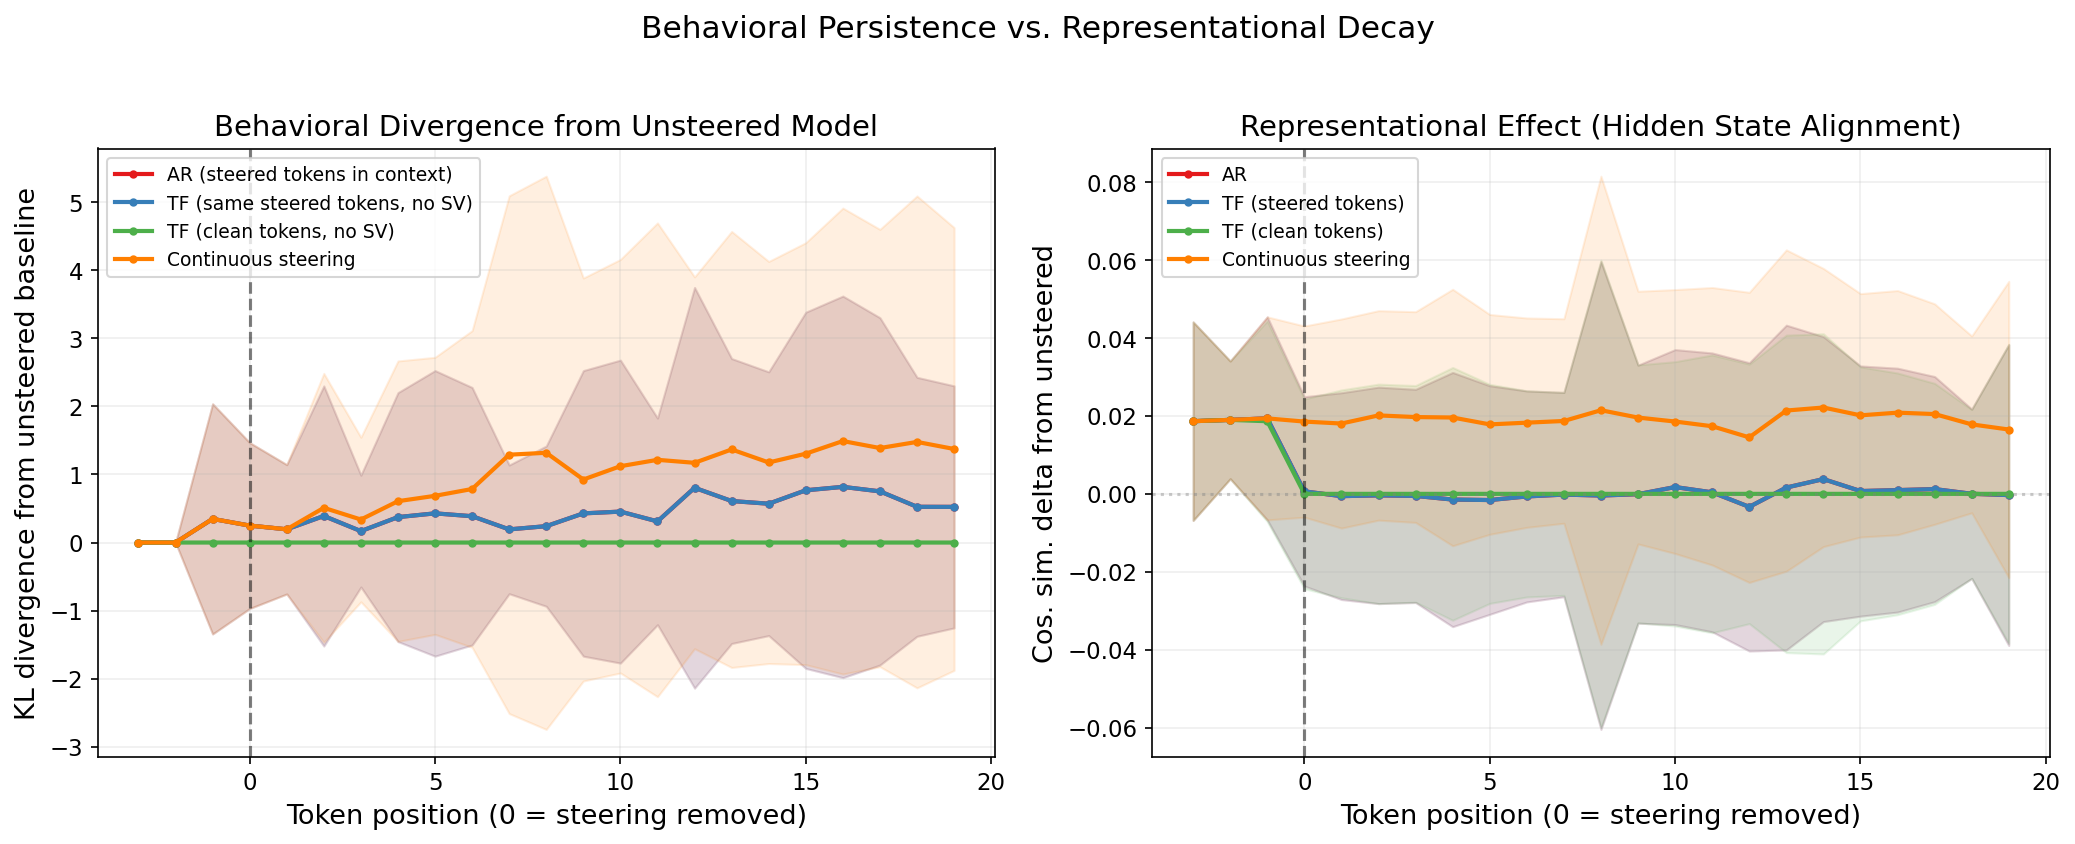
\includegraphics[width=0.95\linewidth]{figures/key_finding_behavioral_vs_representational.png}
    \caption{Dissociation between representational and behavioral effects after
    steering removal. \figleft Cosine similarity delta drops to zero within one
    step (representational decay). \figright KL divergence from the unsteered
    baseline remains elevated under \AR (behavioral persistence through steered
    tokens in context) but is zero under \TFclean (no steered tokens in
    context). This confirms that behavioral persistence operates entirely
    through the autoregressive token feedback loop.}
    \label{fig:behavioral}
\end{figure}

\subsection{Experiment 3: Ablations}
\label{sec:ablations}

We conduct ablations across three dimensions to test the generality of
instantaneous decay. All ablations use the positive sentiment direction.

\para{Layer ablation.}
\Tabref{tab:ablations} (top) shows results for injection at layers 8, 16, 24,
and 32. Earlier layers produce larger steering effects during application
(layer~8: $\Delta\text{cos} = 0.039$; layer~32: $\Delta\text{cos} = 0.010$),
consistent with prior findings that early-to-middle layers are most
effective for steering~\citep{turner2023actadd}. However, all layers show
instantaneous decay at position~0, with post-removal deltas indistinguishable
from zero.

\para{Multiplier ablation.}
\Tabref{tab:ablations} (middle) varies the multiplier $\alpha$ from 1.0 to 5.0.
The delta during steering scales proportionally with the multiplier ($\alpha=1$:
$0.006$; $\alpha=5$: $0.030$), but all multiplier strengths show the same
instantaneous decay. Even at $5\times$ the default strength, the perturbation
is fully absorbed within one step.

\para{Duration ablation.}
\Tabref{tab:ablations} (bottom) varies the steering duration $K$ from 1 to 10
tokens. The delta during steering is constant at ${\sim}0.019$ regardless of
duration, and all durations show instantaneous decay at position~0. Steering for
10~tokens does not create any accumulated effect relative to steering for a
single token.

\begin{table}[t]
    \centering
    \caption{Ablation results for the positive sentiment direction. We report
    $\Delta$cos during steering and at the first post-removal position (pos~0).
    Regardless of layer, multiplier, or duration, decay is instantaneous.
    Default values are layer~24, $\alpha = 3.0$, $K = 3$.}
    \label{tab:ablations}
    \begin{tabular}{@{}llrr@{}}
        \toprule
        Parameter & Value & During steering & At pos~0 \\
        \midrule
        \multirow{4}{*}{Layer ($\ell$)}
        & 8 (early)  & $0.039$ & ${\sim}0.000$ \\
        & 16         & $0.029$ & ${\sim}0.000$ \\
        & 24 (mid)   & $0.019$ & ${\sim}0.000$ \\
        & 32 (late)  & $0.010$ & ${\sim}0.000$ \\
        \midrule
        \multirow{4}{*}{Multiplier ($\alpha$)}
        & 1.0 & $0.006$ & ${\sim}0.000$ \\
        & 2.0 & $0.010$ & ${\sim}0.000$ \\
        & 3.0 & $0.019$ & ${\sim}0.000$ \\
        & 5.0 & $0.030$ & ${\sim}0.000$ \\
        \midrule
        \multirow{4}{*}{Duration ($K$)}
        & 1  & $0.019$ & ${\sim}0.000$ \\
        & 3  & $0.019$ & ${\sim}0.000$ \\
        & 5  & $0.019$ & ${\sim}0.000$ \\
        & 10 & $0.019$ & ${\sim}0.000$ \\
        \bottomrule
    \end{tabular}
\end{table}

\Figref{fig:ablations} visualizes these ablations together. The key observation
is that while the magnitude of the steering effect during application varies
substantially across conditions, the decay pattern is invariant: all conditions
show a step-function drop to zero at position~0.

\begin{figure}[t]
    \centering
    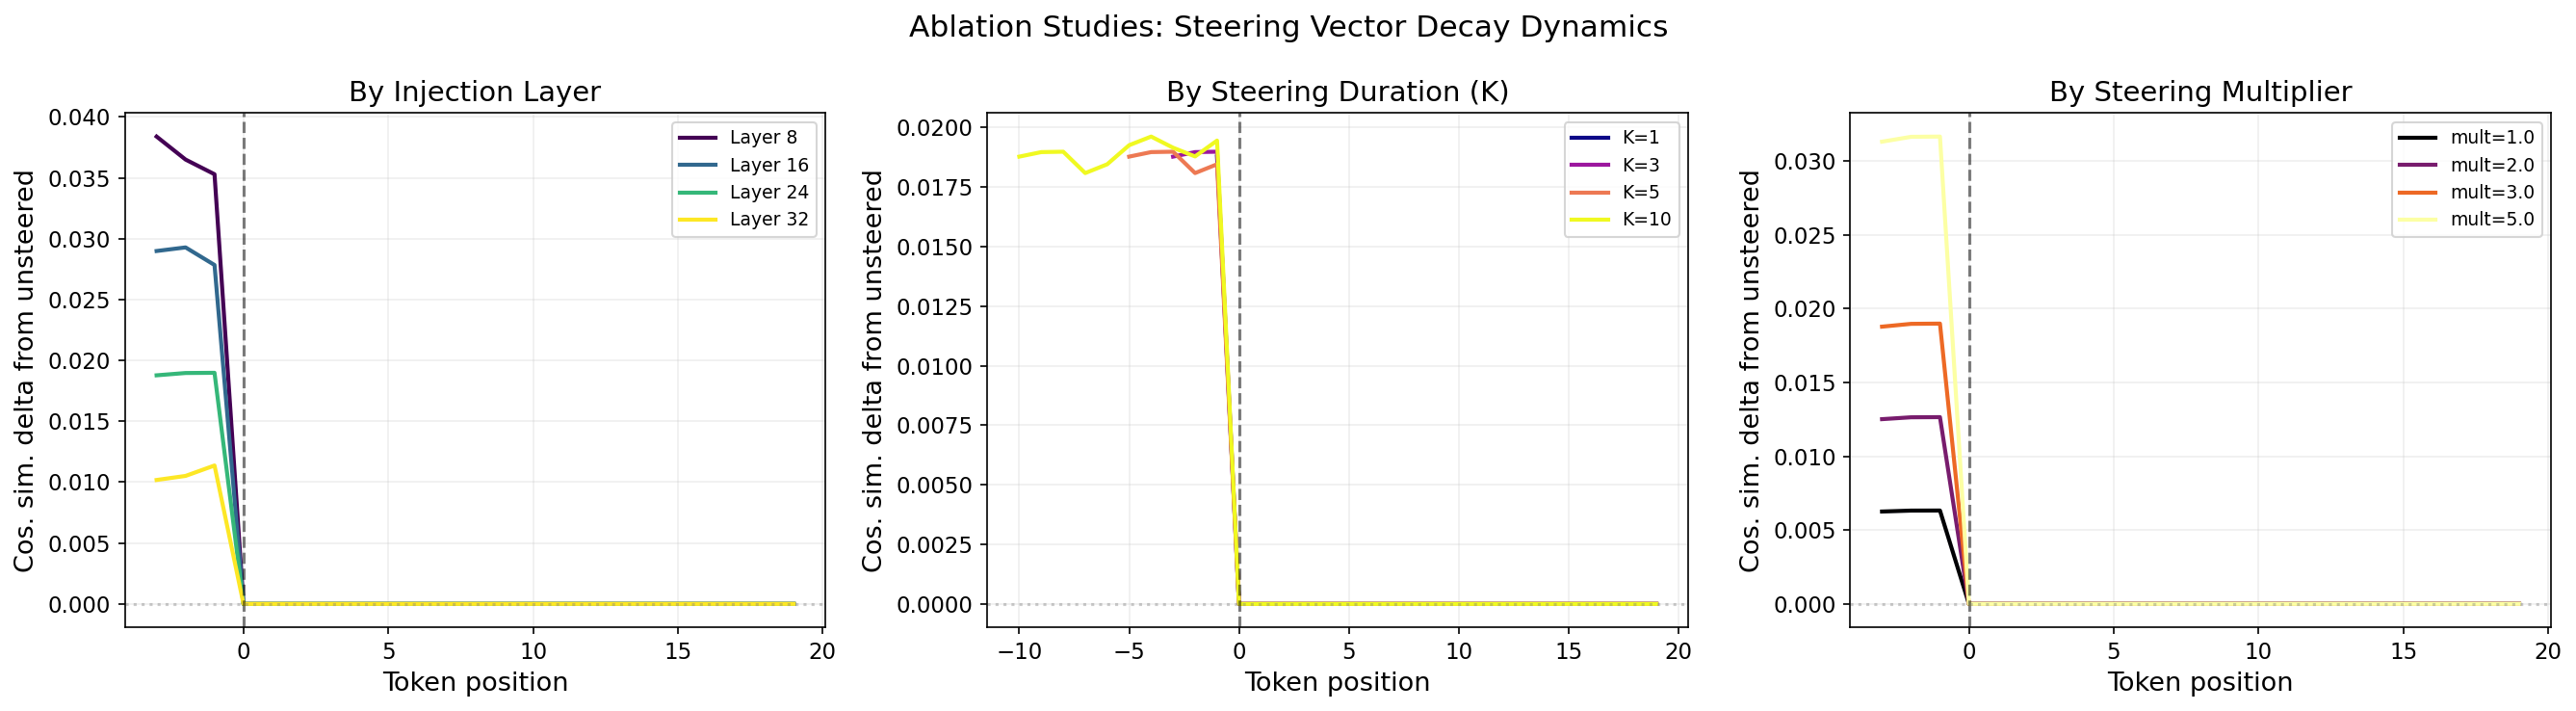
\includegraphics[width=0.95\linewidth]{figures/ablation_summary.png}
    \caption{Ablation results across layers, multiplier strengths, and steering
    durations. While the magnitude of the steering effect during application
    varies across conditions (\figleft: earlier layers produce larger effects;
    \figcenter: larger multipliers produce proportionally larger effects),
    all conditions show the same instantaneous decay at position~0
    (\figright: duration has no effect on either magnitude or decay).}
    \label{fig:ablations}
\end{figure}
